\documentclass{article}

% ------------------------------------ %
%             Document Info            %
% ------------------------------------ %

\usepackage{../../../LaTeX-Preamables/Assign}

\begin{document}
\newcommand{\documentcourse}{COMP2121}
\newcommand{\documentnumber}{5}

% ------------------------------------ %
%                Header                %
% ------------------------------------ %

\begin{minipage}{0.07\textwidth}
    
\includegraphics[width=\linewidth]{../../../LaTeX-Preamables/LaTeX-Templates/HKULOGO256.png}
\end{minipage}
\hspace{0.02\textwidth}
\begin{minipage}{0.55\textwidth}
    \documentcourse

    Assignment \documentnumber

    SID: 3036268218
\end{minipage}
\begin{minipage}{0.35\textwidth}
    \begin{flushright}
        Jax

        \jobname.pdf

        \today
    \end{flushright}
\end{minipage}

\vspace{0.5cm}

\hrule

% ------------------------------------ %
%                Content               %
% ------------------------------------ %

\section*{Question 1}
\hrule
\vspace{0.5cm}

\begin{enumerate}[label=(\alph*)]

    \item (10 marks) Consider the simple graph whose vertex set is $V = \{1, 2, \dots, 20\}$ and whose edge set is defined by the condition that $\{a, b\} \in E(G)$ if and only if $a + b$ is odd. Investigate whether it (i) is connected, (ii) is bipartite, (iii) has an Euler path or cycle, and (iv) has a Hamilton path or cycle.

    \item (10 marks) A simple undirected graph is called regular if every vertex of the graph has the same degree.
          Let $G = (V, E)$ be a connected simple undirected regular graph with $|E| = 22$ edges. What are the possible orders of $G$, i.e., what are the possible values of $|V|$?
\end{enumerate}

\subsection*{Solutions to question 1}

\begin{enumerate}[label=(\alph*)]
    \item
          \begin{enumerate}[label=(\roman*)]
              \item  Consider the condition $\{a,b\} \in E(G)\ iff\ a+b\ odd$. $a=1$ is connected to all $b$ such that $b$ is even up till $20$. Then, $a=2$ is connected to all $b$ such that $b$ is odd up till $19$. As $a=1$ is connected to $b=2$, $a=1$ is connected to all even numbers and $b$ is connected to all odd numbers, thus, the graph is connected.
              \item A bipartite graph is a graph that can be divided into two sets of nodes, called a bipartition $(V_1, V_2)$, such that no two nodes in the same set are connected. In this case, $V_1$ is the set of odd numbers and $V_2$ is the set of even numbers. The condition $\{a,b\} \in E(G)\ iff\ a+b\ odd$ implies that $a$ and $b$ are in different sets. Thus, the graph is bipartite.
              \item If all nodes have an even degree, then the graph has an Euler cycle. As each odd node is connected to all even nodes, and each even node is connected to all odd nodes, each node has a degree of $10$, which is even. Thus, the graph has an Euler cycle. As all degrees are even, there is no Eular path.
              \item Note the graph is a simple, \textbf{complete} bipartite graph. We know that a complete bipartite graph $K_{m,n}$ has a Hamiltonian cycle if and only if $m=n$. In this case, $m=10$ and $n=10$, thus the graph has a Hamiltonian cycle. (and thus a path)
          \end{enumerate}
    \item Using the handshaking theorem $2|E|=\sum_{v\in V}deg(v)$. As $G$ is regular, thus, $44=|V|*d, |V| \leq 22, d \leq |V| - 1$ (connected, simple). The candidate values are:
          \begin{itemize}
              \item $|V|=2, d=22$ (not simple)
              \item $|V|=4, d=11$ (not simple)
              \item $|V|=11, d=4$ (valid)
              \item $|V|=22, d=2$ (valid)
          \end{itemize}
          Hence, $|V| \in \{11, 22\}$.
\end{enumerate}

\section*{Question 2}
\hrule
\vspace{0.5cm}

\begin{enumerate}[label=(\alph*)]
    \item (8 marks) At the Wizardry department in Hogwarts School, there are seven committees $C_1 - C_7$ consisting of members as indicated:

          $C_1 = \{D, N, L\}, C_2 = \{L, M, H\}, C_3 = \{M, S\},$

          $C_4 = \{D, G\}, C_5 = \{H, T\}, C_6 = \{H, N, G\}$

          and $C_7 = \{T, L, S\}$. (Simplified)

          The committees need to schedule times for three-hour meetings in a particular week. Since each member must be present at each of his or her committee meetings, the meeting times need to be scheduled carefully to not clash with each other. Determine the fewest number of meeting times that need to be scheduled so that all the committees can meet in the week.
    \item (10 marks) A connected graph $G$ is said to be chromatically $k$-critical if $\chi(G) = k$, but for every edge of $G$, the chromatic number of the graph obtained by deleting this edge from $G$ is $k-1$. Show that if $G$ is a chromatically $k$-critical graph, then the degree of every vertex of $G$ cannot be smaller than $k-1$.
    \item (10 marks) A polyhedron is a geometric object consisting of flat polygonal faces joined at edges and vertices. Convex polyhedra have the property that any line segment connecting two points on the polyhedron must be entirely contained within the polyhedron. Furthermore, a regular polyhedron is one in which all the faces are congruent (identical in shape and size) regular polygons (all angles congruent and all edges congruent) and the same number of faces meet at each vertex.
          How many convex regular polyhedra are there such that each face is a triangle?
    \item (8 marks) Fig. 1 depicts the standard pattern covering a football using both hexagons (6-sided polygons) and pentagons (5-sided polygons).
          When using this pattern to cover the surface of a football, what are the number of hexagons and the number of pentagons? Show how these numbers are calculated.

          
\includegraphics[width=0.2\textwidth]{5-fig-1.png}
\end{enumerate}

\subsection*{Solutions to question 2}

\begin{enumerate}[label=(\alph*)]
    \item Model the problem as a graph. Each node is a committee, and an edge represents a common member between two committees:

          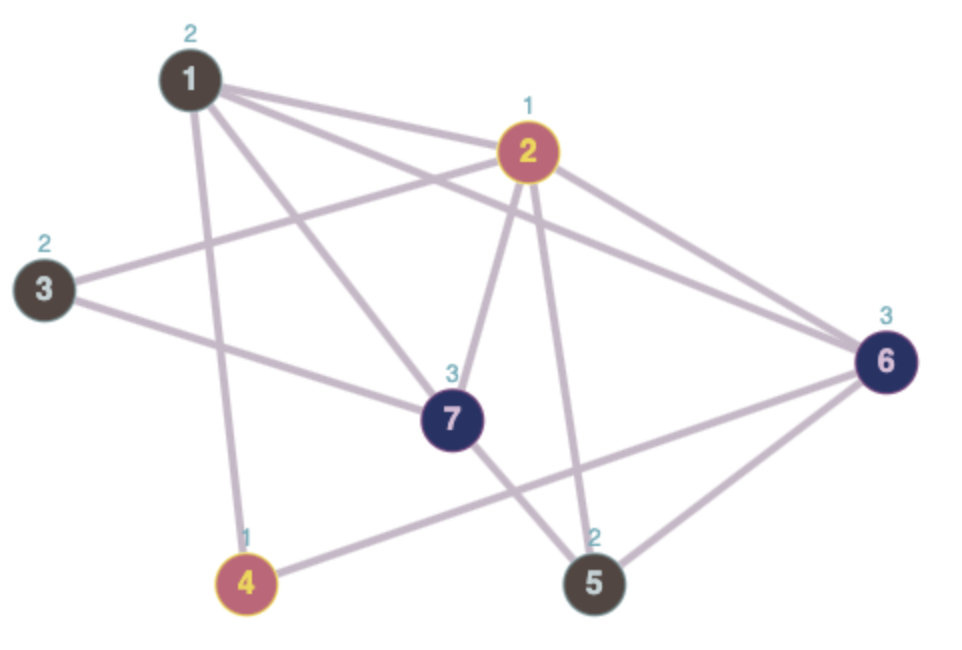
\includegraphics[width=0.5\textwidth]{5-2-a.png}

          %   http://graphonline.top/?graph=pAefVojsxcUBBsxK

          Hence, by coloring number of time slots needed is 3.

    \item Given $\chi(G)=k,\quad \chi(G-e) = k-1 \forall e \in E$, we have to proof that $deg(v) \geq k-1$ for all $v \in V$. Assume the contrary, that is, there exists a vertex $v$ such that $deg(v) < k-1$. Removing this vertex can lead to $\chi(G-v) \leq k-1$ colors. We know that the excessive coloring of neighbors of $v$ must be at most $deg(v) < k-1$, that is $k-2$. So adding the node $v$ back gives $\chi(G) \leq k-1$, contradicting the $chi(G)=k$ condition. Hence, $deg(v) \geq k-1$ for all $v \in V$.
    \item We can solve this problem using Euler's formula.
          \begin{itemize}
              \item As each face is a triangle and each edge is shared by two faces, $|R| = \frac23 |E|$.
              \item By the property of polyhedra, each node is shared by a constant amount of faces, which is the degree of the node. By handshaking theorem, $2|E| = |V| \times d$, where $d$ is the constant degree of nodes mentioned.
          \end{itemize}
          \begin{align*}
              |R| = |E| - |V| + 2                                                           \\
              \frac{2|E|}{3} - |E| + \frac{2|E|}{d} & = 2                                   \\
              |E|(\frac{2}{3} - 1 + \frac{2}{d})    & = 2                                   \\
              |E|                                   & = \frac{2}{\frac{2}{d} - \frac{1}{3}} \\
              \because \frac{2}{d} - \frac{1}{3}    & > 0,\quad d < 6                       \\
              \therefore d                          & = 3,4,5                               \\
          \end{align*}
          Therefore, the the count required is 3.
    \item We can solve this problem using Euler's formula (again). Let $p$ be number of pentagons, and $h$ be number of hexagons. Hence, number of regions $|R| = p + h$. Then, we can model the problem as a graph.

          \begin{itemize}
              \item  Each pentagon has 5 nodes and edges, and hexagons 6 nodes and edges. $|E| = \frac{5p + 6h}{2}$, as each edge is counted twice.
              \item From the image, we can see that each vertex is shared by 3 faces, thus $|V| = \frac{5p + 6h}{3}$. By Euler's formula:
          \end{itemize}
          \begin{align*}
              |R| = |E| - |V| + 2                                 \\
              \frac{5p + 6h}{3} - \frac{5p + 6h}{2} + p + h & = 2 \\
              \frac{10p + 12h - 15p - 18h + 6p + 6h}{6}     & = 2 \\
              \frac{p}{6}                                   & = 2 \\
              p                                             & =12 \\
          \end{align*}

          As there are $12$ pentagons, there are $5p = 60$ nodes. $60 = \frac{5p + 6h}{3}$, thus $h = 20$. Hence, there are $12$ pentagons and $20$ hexagons.
\end{enumerate}


\section*{Question 3}
\hrule\hrule
\vspace{0.5cm}

\begin{enumerate}[label=(\alph*)]
    \item (12 marks) Landau is an old-fashioned hands-on electrical engineer and has designed a rotating drum consisting of $2^k$ sectors as shown in the Fig. 2 for the case $k = 3$. He wants to label each sector with either a 0 or a 1 so that each $k$-bit string as read consecutively clockwise on the drum is different (three readers are shown in the figure for the case $k = 3$). As the drum rotates in a clockwise manner, the $k$ bits will be read off at the positions indicated in the figure (essentially, Landau is looking for a $2^k$-bit string that allow him to have all $k$ different readings).

          Your task is to help Landau assign a 0 or a 1 to each of the $2^k$ sectors to satisfy his requirement. Use a suitably defined directed pseudograph and an Euler circuit on the graph to help Landau solve his problem.

          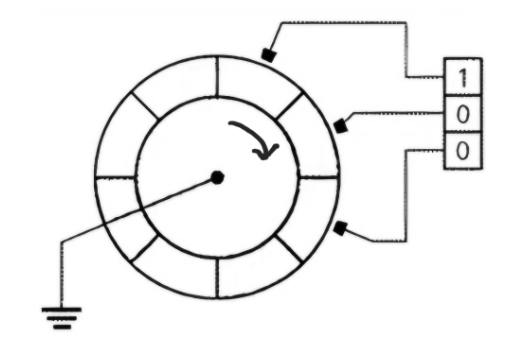
\includegraphics[width=0.3\textwidth]{5-fig-2.png}

          \textit{The sign depicts a rotating drum consisting of 8 sectors. It is possible to label each of the 8 sectors with a 0 or a 1 so that the reader reads each of the eight bit strings 000, 001, 010, 011, 100, 101, 110, 111 as the drum rotates.}

    \item (14 marks) Suppose $G = (V, E)$ is a simple undirected graph, where $n = |V| \geq 3$ and $m = |E|$. The purpose of this question is to find the maximum possible value of $m$ (in terms of $n$) such that $G$ has no Hamiltonian cycle.

          \begin{enumerate}[label=(\roman*)]
              \item For some value of $m$ that will be decided later, suppose a graph $G$ contains $m + 1$ edges. The goal is to show that $G$ must contain a Hamiltonian cycle. We shall prove this by contradiction. Suppose there exists two vertices $u$ and $v$ in $V$ such that there is no edge in $G$ between $u$ and $v$.

                    Based on Dirac’s or Ore’s Theorems on Hamiltonian cycles, what assumption should be made regarding $u$ and $v$ to set up the contradiction proof?

              \item Suppose that in the graph $G$ in part (i), vertices $u$ and $v$ (together) with their incident edges are removed. Give a lower bound on the number of remaining edges in terms of $n$ and $m$.

              \item Determine a value of $m$ (in terms of $n$) to reach a contradiction.

              \item Prove that the value of $m$ you choose in the previous part is optimal. In other words, construct a graph $G$ with $n$ vertices and $m$ edges such that $G$ has no Hamiltonian cycle.
          \end{enumerate}
\end{enumerate}

\subsection*{Solutions to question 3}

\begin{enumerate}[label=(\alph*)]
    \item A key property is that for a string of $k$ bits, there are $2^k$ possible strings. Define the directed pseudograph $G$ as follows:
          \begin{itemize}
              \item Each vertex is one of the $k-1$-bit strings. (total $2^{k-1}$ vertices)
              \item An edge exists if for pairs of nodes $(u,v)$, the first bit of $v$ is the same as the last bit of $u$. (total $2^k$ edges)
          \end{itemize}
          Notice that for each node, the in-degree is 2 and the out-degree is 2, because we can add a 0 or a 1 to the end of the string. Hence, the graph has an Euler Circuit (all nodes have same in and out degree). The circuit can be read off as the required string.

          Example $k=3$ graph:

          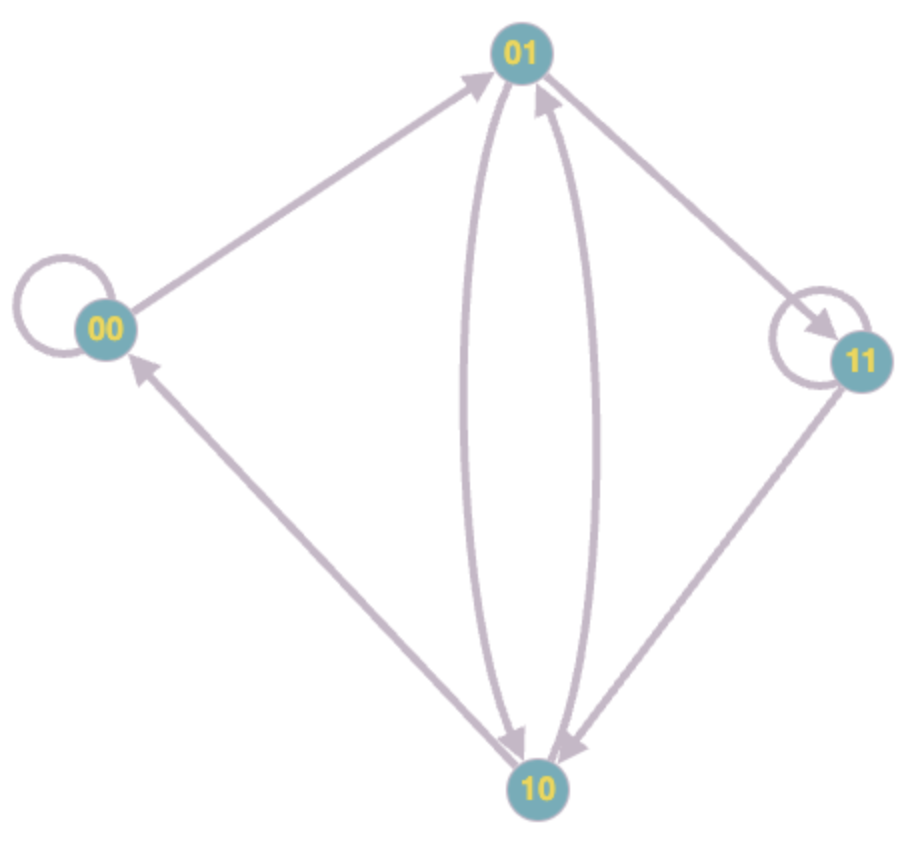
\includegraphics[width=0.3\textwidth]{5-3-a.png}
    \item
          \begin{enumerate}[label=(\roman*)]
              \item $deg(u)+deg(v)< n$ (Goal is to fail the ore's theorem's condition)
              \item By the above condition, the maximum number to be removed is at most $n-1$. Hence, lower bound on number of edges remaining is $m+1 - (n-1) = m - n + 2$.
              \item Removing two nodes: $|V|=n-2$. We can find the possible number of edges by $\binom{n-2}{2}$. Hence:
                    \begin{align*}
                        m - n + 2 & \leq \binom{n-2}{2}       \\
                        m - n + 2 & \leq \frac{(n-2)(n-3)}{2} \\
                        m         & \leq \frac{(n-1)(n-2)}{2} \\
                    \end{align*}
                    Hence, the maximum value we will use is $m=\frac{(n-1)(n-2)}{2}$.
              \item We can show that our $m$ is optimal by using a complete $K$ graph. As the number of edges in $K_k$ is $\frac{k(k-1)}{2}$, we want $m=\frac{(k-1)(k-2)}{2} \implies k = n-1$. For a $K_{n-1}$ graph, there are $m$ edges, and $n-1$ vertices. This means that if we add a final node $n_0$ to the graph, it is not connected to the rest of the graph, thus the graph with $m$ edges and $n$ vertices has no Hamiltonian cycle.
          \end{enumerate}
\end{enumerate}
\section*{Question 4}
\vspace{0.5cm}\hrule
\vspace{0.5cm}

\begin{enumerate}[label=(\alph*)]
    \item (10 marks) Let $G = (V, E)$ be a $k$-regular (meaning each vertex has degree $k$) bipartite simple undirected graph with equal sized bipartitions, for some $k \geq 1$. That is, $V = V_1 \cup V_2$ with $V_1 \cap V_2 = \emptyset$ and $|V_1| = |V_2|$, and all edges in the graph connect vertices in $V_1$ to vertices in $V_2$. Use Hall’s Marriage Theorem to show that $G$ has a perfect matching.

    \item (8 marks) At InGen Technologies, Edmund has received three shipments that contain a total of seven different DNA samples. To avoid contamination, for all $1 \leq k \leq 5$ sample $k$ cannot be stored in the same ultra-low temperature freezer as sample $k + 1$ or sample $k + 2$.

          Determine the minimum number of separate ultra-low temperature freezers that Edmund will need to store the seven DNA samples.
\end{enumerate}

\subsection*{Solutions to question 4}

\begin{enumerate}[label=(\alph*)]
    \item Given each vertex has degree k, $G=K_{k,k}$. The theorem states that if $|N(W)| \geq |W|$ for all $W \subseteq V_1$, then there exists a perfect matching. As $G$ is bipartite, $|N(W)| = k|W|$. Thus, $k|W| \geq |W| \implies |N(W)| \geq |W|$, and so therefore $G$ has a perfect matching.
    \item The following pairs are illegal: $(1,2), (1,3), (2,3), (2,4), (3,4), (3,5), (4,5), (4,6), (5,6), (5,7)$. First, draw graph with these edges:

          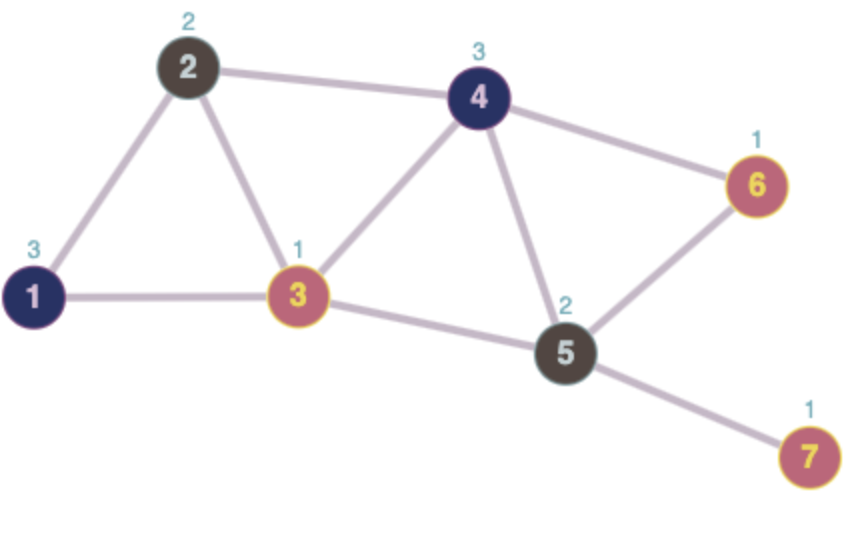
\includegraphics[width=0.5\textwidth]{5-4-b.png}
          % http://graphonline.top/?graph=rjbfzVkjdncQMVWa

          As minimum coloring is 3, we need 3 freezers.
\end{enumerate}
\end{document}
